% Dossier d'Initialisation - H4413

\documentclass[twoside]{article}
\usepackage{hyperref}


\usepackage{graphicx}
\usepackage{subfig}
\usepackage{placeins}


% Unicode encoding  
\usepackage[utf8x]{inputenc}


% Colorfull Text
\usepackage{xcolor}


% \euro
\usepackage{eurosym}


% Language settings:
\usepackage[french]{babel}

\usepackage[T1]{fontenc}


% Tables
\usepackage{array}
\usepackage{longtable}


% Hyperrefferences  
\usepackage{hyperref}


\title{Dossier d'Initialisation}
\author{H4413}
% Page layout settings
\usepackage{geometry}
\geometry{
	a4paper,  % 21 x 29,7 cm
	body={160mm,240mm},
	left=30mm, 
	top=25mm,
	headheight=7mm, 
	headsep=4mm,
	marginparsep=4mm,
	marginparwidth=27mm
}


% Spacing:
\usepackage{setspace}


% Headers and footers:
\usepackage{fancyhdr}
\pagestyle{fancy}
          \fancyhf{}
          \fancyfoot[LE,RO]{\textcolor[gray]{0.3}{\thepage}}
          % Rulers width
          \renewcommand{\footrulewidth}{.3pt}
          \renewcommand{\headrulewidth}{.0pt}
\fancyfoot[LO,RE]{\textcolor[gray]{0.3}{H4413}}
\fancyfoot[CO,CE]{\textcolor[gray]{0.3}{Dossier d'Initialisation}}


% Vars & functs
% Paths
\newcommand\PIXPATH{./docs/pics}
\newcommand\SRCPATH{./docs/src}

% Object:
\newcommand\Object{Dossier d'initialisation du projet PLD}

% End of line(forced):
\newcommand\el{\hfill\\}

% Lists design:
\renewcommand{\labelitemi}{$\diamond$}
\renewcommand{\labelenumii}{\arabic{enumi}.\arabic{enumii}}


% Begining of the document
\begin{document}

	%Including all the files:

    % Fichier ./docs/tex/00.a.premiere_page.tex

% Front Page 

% Title:
\maketitle

\thispagestyle{empty}

\hfill\\
\vfill

% Picture

\begin{center}
    
\includegraphics[width=5cm]{\PIXPATH/frontPage}
\end{center}

\section*{Objet}
\Object

    % Fichier ./docs/tex/00.b.suivi.tex

% Suivi du document

% Modifications
\section*{Modifications du document}

\begin{center}
\begin{longtable}{|m{14mm}|m{36mm}|m{36mm}|m{60mm}|}
\hline
Version & Auteur & Date & Modification\endhead \hline
% Version
0
& % Auteur
Raphaël Lizé
& % Date
7 janvier 2011
& % Modification
Création
\\\hline
% Version
0.1
& % Auteur
Quentin Villers
& % Date
18 janvier 2011
& % Modification
Première Version
\\\hline
% Version
0.2
& % Auteur
Quentin Villers
& % Date
20 janvier 2011
& % Modification
Corrections mineures
\\\hline
% Version
0.3
& % Auteur
Raphaël Lizé
& % Date
21 janvier 2011
& % Modification
Mise en page
\\\hline
% Version
1
& % Auteur
Raphaël Lizé
& % Date
21 janvier 2011
& % Modification
RC1
\\\hline
% Version
1.1
& % Auteur
Raphaël Lizé
& % Date
21 janvier 2011
& % Modification
Corrections mineures
\\\hline
\end{longtable}
\end{center}

% Validations

\section*{Vérifications et validations du document}

\begin{center}
\begin{longtable}{|m{15mm}|m{36mm}|m{36mm}|m{60mm}|}
\hline
 & Responsable & Date & Remarques\endhead \hline
% Validé/vérifié par
Validé
& % Responsable
Quentin Villers
& % Date
21 janvier 2011
& % Remarques
\\\hline
% Validé/vérifié par
Vérifié
& % Responsable
Raphaël lizé
& % Date
21 janvier 2011
& % Remarques
Le document est livrable
\\\hline
\end{longtable}
\end{center}

\pagebreak

    % Fichier ./docs/tex/00.c.toc.tex

% Table of contents 
\tableofcontents
\vfill
\pagebreak

    % Fichier ./docs/tex/1-ObjetsDuProjetEtContexte.tex

\section{Objet du projet et contexte}
%1-2 pages
%L’objet du projet
%Le contexte général du projet ; son positionnement éventuel dans un projet plus vaste ; synthèse
%des phases antérieures si il y a lieu.
%Son positionnement dans le cycle de vie général du développement des système d’information (
%identification du type de phase à laquelle correspond le projet ; ex : étude préalable,
%spécification d’interface, étude d’architecture technique, réalisation, test, ....)

\subsection{Objet du projet GSTP}
Le projet est une étude préalable de la conception et de l'automatisation
du système d'information du domaine \textsl{gestion du matériel} dans l'entreprise 
GSTP qui est spécialisée dans les activités de terrassement et génie civil.\\

Le but du dossier d'initialisation est de déterminer le périmètre du projet
SI et sa faisabilité, c’est-à-dire de définir ce qui sera inclu
dans le projet, ce qui ne le sera pas et si le projet doit bien être
lancé.\\

D’une part, on estime si les bénéfices attendus seront en proportion des
investissements engagés et du coût prévisionnel du projet SI.  D’autre
part, l’étude préalable détermine également si l’entreprise GSTP est
bien en mesure de mener ce projet à son terme. On cherche en particulier
à savoir si elle dispose des compétences, des ressources et des fonds
nécessaires.\\

On peut dire pour résumer rapidement que le projet consister à urbaniser le
SI de la société GSTP.


\subsection{Contexte général du projet : présentation de l'entreprise GSTP}

La société GSTP est une SA au capital de 500 M\euro. Elle a à gérer un parc
matériel d'une valeur totale de 300 M\euro\ et un stock de pièces de
rechanges d'une valeur totale de 100 M\euro.

\subsubsection{Secteur d'activité}
Le projet prend place dans le monde du bâtiment et travaux publiques (GSTP
signifie Génie et Services dans Monde du Bâtiment et Travaux Publiques).


\subsubsection{Organigramme}
L'entreprise est bien structurée et le rôle des différentes entités est clairement défini.\\
On présente ici l'organigramme de la direction du matériel, sur laquelle
portera le projet.\\

\begin{center}
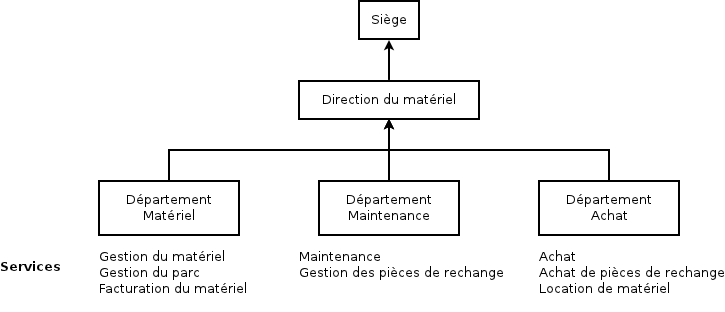
\includegraphics[width=14cm]{\PIXPATH/orga_dir_mat}\hfill\\
\end{center}

La direction du matériel est placée sous la direction de la direction générale
de la société GSTP. Elle comprend trois départements :\\

\begin{description}

\item[Département matériel:] il gère l'exploitation du matériel de la
société sur les différents chantiers qu'elle mène;
\item[Département maintenance:] il s'occupe des opérations de maintenance
ordinaires ou exceptionnelles entreprises sur le matériel;
\item[Département achat:] il a pour charge le renouvellement du parc et
l'achat de nouveaux matériels si nécessaire ; il s'occupe également des
achats de pièces de rechanges.

\end{description}


\subsubsection{Organisation structurelle}

La structure de l'entreprise est basée sur la division siège/chantier :
\begin{description}
\item[Siège]\hfill\\ 
Entité unique où sont regroupés les divers comités de direction de l'entreprise
(DG, DRH, DFC, etc.)

\item[Chantier]\hfill\\
Multiples (la société GSTP genre environ 40 chantiers en même temps),
ils sont répartis dans un rayon de 500 km autour du siège.
Les chantiers jouissent d'une certaine autonomie de fonctionnement et
financière par rapport au siège. Les chantiers sont planifiés par la DTEM
au siège de la société. Enfin, le chantier est décrit par une multitude
d'attributs du point de vue gestion (code, nom, localisation, etc.).
\end{description}


\subsubsection{Equipement informatique}

Le siège est bien équipé en matériel informatique. En revanche, 
L'équipement des chantiers en matériel informatique est disparate (un tiers
des chantiers est équipé) ; toutefois, l'ensemble sera équipé sur un horizon de
dix mois, ce qui permet d'envisager le projet de manière sereine de ce côté
là.


\subsection{Identification des secteurs de l'entreprise impactés par le projet}

\subsubsection{Activités de l'entreprise}

L'activité principale (travaux publiques) de l'entreprise ne va pas
vraiment être impactée par le projet. En revanche, la manière dont
l'entreprise gère son matériel va se trouver transformée.


\subsubsection{Directions et services}

Au vu de l'objet du projet (automatisation du SI du domaine \textsl{gestion du
matériel}), on peut dire que la principale direction de l'entreprise touchée
par le projet sera la direction du matériel. Tous les départements de cette
direction seront également touchés par le projet.\\
La manière dont les chantiers gèrent le matériel sera également impactée.


\subsubsection{Processus et procédures stratégiques}

Toutes les procédures liées au matériel employé par la société seront
touchées par le projet. Cela comprend les procédures suivantes :
\begin{itemize}
\item Renouvellement du matériel;
\item Affectation;
\item Facturation;
\item Maintenance.
\end{itemize}


    % Fichier ./docs/tex/2-Livrables.tex

% 2
\section{Livrables}
%3-4 pages
%Liste et plans types des documents et des composants logiciels demandés (directement les
%annexes G et H si elles sont peu importantes

\subsection{Dossier d'initialisation et plan d'assurance qualité}

Ces documents vont assurer le lancement du projet et permettre d'organiser
la gestion des ressources le plus efficacement possible pour le dossier d'initialisation.
Le plan d'assurance qualité va permettre de définir le cadre du projet, c'est à dire les outils utilisés et les modalités de contrôle notamment. 

\subsection{Dossier d'expression des besoins}

Le dossier d'expression des besoins va comporter l'analyse de l'existant
de la société GSTP. Les équipes se formeront ensuite sur l'état de l'art
mis en place chez la concurrence (Vinci par exemple). L'ensemble des deux
analyses permettra de fournir les spécifications du système d'information cible
au travers de la modélisation faite par nos outils comme ARIS. 

\subsection{Dossier des solutions}

Le dossier des solutions va comprendre deux principaux volets :
\begin{itemize}
    \item La spécification d'une solution spécifique comprenant des rapports
        les dimensions organisationnelle et informatique de la solution;
    \item La spécification d'une solution standard utilisant l' ERP SAP et une
        modélisation avec l'outil ARIS.
\end{itemize}

\subsection{Dossier des choix}

Ce dossier sera un résumé de la partie précédente, il nous permettra de choisir
entre les deux solutions proposées, c'est à dire la solution spécifique et la
solution standard en fonction de critères de décision. 

\subsection{Restitution et dossier bilans}

Cette partie concernera à la fois la présentation finale prévue en semaine 10
ainsi que les dossiers bilans qui feront la synthèse du travail fourni par l'équipe.

\subsection{Récapitulatif des dates butoirs}

\begin{longtable}{|l|l|}
\hline
Livrables& Date\\
\endhead \hline
Dossier d'initialisation& 21/01/2011\\
\hline
Plan d'assurance qualité& 21/01/2011\\
\hline
Étude des besoins& 11/02/2011\\
\hline
Dossier des solutions& 18/02/2011\\
\hline
Dossier des choix& 25/02/2011\\
\hline
Restitution et bilans& 11/03/2011\\
\hline
Présentation&  11/03/2011\\
\hline
\end{longtable}


    % Fichier ./docs/tex/3-IdentificationDesActivites.tex

%3
\section{Identification des activités et des tâches}
%Liste des ACTIVITES et des TACHES
%1 tâche = 1 étudiant et 1 semaine
%1 étudiant peut avoir plusieurs tâches la même semaine (en parallèle)
%PLAN DE CHARGES ( voir document spécifique )
%PLANNING ( DIAGRAMME DE GANTT )
%à l’aide d’un outil de gestion de projet : MS Project

\subsection{Schéma de déroulement général}

Selon le planning établi lors de la partie précédente, nous obtenons la liste des livrables.

\begin{center}
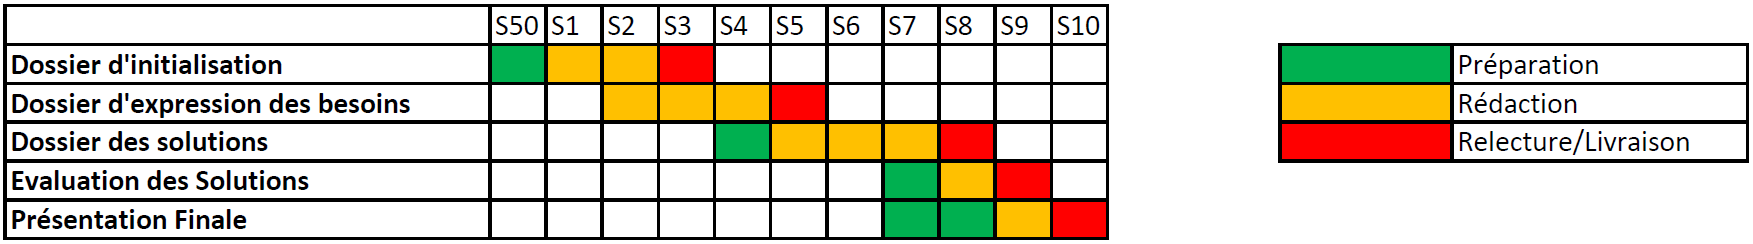
\includegraphics[width=17cm]{\PIXPATH/gantt}\hfill\\
\end{center}

\vfil
\pagebreak
\subsection{Liste des tâches par personne}

Il s'agit d'une liste des tâches avec un \textsl{timing} raisonnable.
Une révision et un affinage sera produit chaque semaine par le chef de projet
en amont de la séance du vendredi.

\subsubsection{Quentin Villers}

Les tâches d'encadrement comprennent des entrevues individuelles pour conduire l'équipe. 
Elles s'appliquent aussi bien au responsable qualité qu'aux membres de l'équipe. 

\begin{longtable}{|l|l|l|}
\hline
Semaine&Durée en H&Tâches\\
\endhead \hline
S00&1&Initialisation\\
\hline
S00&0,5&Réunion\\
\hline
S01&0,5&Réunion\\
\hline
S01&3&Pilotage\\
\hline
S01&3&Rédaction dossier d'initialisation\\
\hline
S02&0,5&Réunion\\
\hline
S02&2&Planification\\
\hline
S02&3&Encadrement\\
\hline
S03&0,5&Réunion\\
\hline
S03&2&Encadrement\\
\hline
S03&0,5&Recette PAQ\\
\hline
S03&1&Recette dossier d'initialisation\\
\hline
S03&0,5&Recette EDB -1\\
\hline
S04&0,5&Réunion\\
\hline
S04&2&Encadrement\\
\hline
S04&0,5&Recette \textsl{benchmarking}\\
\hline
S04&2&Synthèse du document\\
\hline
S05&0,5&Réunion\\
\hline
S05&2&Encadrement\\
\hline
S05&1&Recette dossier EDB complet\\
\hline
S05&1&Synthèse de S5\\
\hline
S06&0,5&Réunion\\
\hline
S06&1&Recette solution spécifique\\
\hline
S06&2&Encadrement\\
\hline
S07&0,5&Réunion\\
\hline
S07&1&Recette solution standard\\
\hline
S07&2&Encadrement\\
\hline
S07&2&Recette modélisation sur ARIS\\
\hline
S08&0,5&Réunion\\
\hline
S08&2&Encadrement\\
\hline
S08&4&Préparation du support de présentation final\\
\hline
S09&2&Répétition présentation\\
\hline
S09&1&Relecture du support de présentation\\
\hline
S09&6&Génération des bilans quantitatifs et qualitatifs\\
\hline
S10&4&Présentation finale\\
\hline
\end{longtable}

\pagebreak
\subsubsection{Raphaël Lizé}

Les tâches mentionnées comme de \textsl{soutien} vont permettre à Raphaël d'homogénéiser
la charge de l'équipe en fonction des difficultés rencontrées lors du travail. 
Ici sont mentionnées principalement les tâches inhérentes au rôle de responsable qualité,
l'adaptation de ces missions sera faite de manière agile.

\begin{longtable}{|l|l|l|}
\hline
Semaine&Durée en H&Tâches\\
\hline
S00&1&Initialisation\\
\hline
S00&0,5&Réunion\\
\hline
S01&0,5&Réunion\\
\hline
S01&3&Rédaction PAQ\\
\hline
S02&0,5&Réunion\\
\hline
S02&1&Gestion GIT\\
\hline
S02&5&Rédaction PAQ\\
\hline
S03&0,5&Réunion\\
\hline
S03&1&Recette PAQ\\
\hline
S03&2&Soutien\\
\hline
S03&1&Recette dossier d'initialisation\\
\hline
S04&0,5&Réunion\\
\hline
S04&2&Soutien\\
\hline
S04&1&Intégration des comptes rendus S2 et S3\\
\hline
S05&0,5&Réunion\\
\hline
S05&1&Aide à la réalisation\\
\hline
S05&2&Spécification de la solution spécifique\\
\hline
S05&1&Recette Dossier EDB complet\\
\hline
S05&0,5&Création modèle document solution spécifique\\
\hline
S06&0,5&Réunion\\
\hline
S06&1&Recette solution spécifique\\
\hline
S06&2&Modélisation ARIS\\
\hline
S06&0,5&Création modèle document solution standard\\
\hline
S07&0,5&Réunion\\
\hline
S07&1&Recette solution standard\\
\hline
S07&2&Modélisation\\
\hline
S07&2&Analyse cohérence des résultats\\
\hline
S08&3&Soutien\\
\hline
S08&0,5&Réunion\\
\hline
S08&0,5&Création modèle document choix de solution\\
\hline
S09&2&Répétition présentation\\
\hline
S09&1&Relecture support de présentation\\
\hline
S09&4&Aider Quentin\\
\hline
S10&4&Présentation finale\\
\hline
\end{longtable}
\vfill
\pagebreak

\subsubsection{Victor Borges}
\begin{tabular}{|l|l|l|l|}
\hline
Semaine&Durée en H&Tâches\\
\hline
"S0"&1&"Initialisation"&\\
\hline
"S0"&"0&5"&"Réunion"\\
\hline
"S1"&"0&5"&"Réunion"\\
\hline
"S1"&3&"Rédaction Dossier Init"&\\
\hline
"S2"&3&"Préparation Formation Benchmarking"&\\
\hline
"S2"&"0&5"&"Réunion"\\
\hline
"S3"&"0&5"&"Réunion"\\
\hline
"S3"&"0&5"&"Formation Benchmarking"\\
\hline
"S3"&2&"Benchmarking"&\\
\hline
"S3"&2&"Conclusion S3 Benchmarking"&\\
\hline
"S4"&"0&5"&"Réunion"\\
\hline
"S4"&3&"Analyse des processus"&\\
\hline
"S5"&"0&5"&"Réunion"\\
\hline
"S5"&3&"Spécification de la solution spécifique"&\\
\hline
"S6"&"0&5"&"Réunion"\\
\hline
"S6"&2&"Fonction GSTP "&\\
\hline
"S6"&1&"Organigramme GSTP"&\\
\hline
"S7"&"0&5"&"Réunion"\\
\hline
"S7"&3&"Modélisation sur ARIS"&\\
\hline
"S8"&"0&5"&"Réunion"\\
\hline
"S8"&3&"Chiffrage solution spécifique"&\\
\hline
"S9"&2&"Répétition présentation"&\\
\hline
\end{tabular}
\vfill

\pagebreak
\subsubsection{Karen Abanto}

Les temps affectés à Karen sont jugés comme plus long. Karen aura plus de travail
personnel pour arriver au niveau de résultat attendu. 
Le chef de projet l'encadrera de façon active.

\begin{longtable}{|l|l|l|}
\hline
Semaine&Durée en H&Tâches\\
\hline
S00&1&Initialisation\\
\hline
S00&0,5&Réunion\\
\hline
S01&0,5&Réunion\\
\hline
S01&3&Rédaction dossier d'initialisation\\
\hline
S02&0,5&Réunion\\
\hline
S02&5&Rédaction EDB - 1 Matériau\\
\hline
S02&2&Conclusion S2\\
\hline
S03&0,5&Réunion\\
\hline
S03&0,5&Formation \textsl{benchmarking}\\
\hline
S03&4&\textsl{Benchmarking}\\
\hline
S04&0,5&Réunion\\
\hline
S04&4&Analyse des dysfonctionnements\\
\hline
S05&0,5&Réunion\\
\hline
S05&4&Spécification de la solution spécifique\\
\hline
S06&0,5&Réunion\\
\hline
S06&4&Configuration SAP\\
\hline
S07&0,5&Réunion\\
\hline
S07&4&Modélisation sur ARIS\\
\hline
S08&0,5&Réunion\\
\hline
S08&4&Choix du projet plus organisation de la suite\\
\hline
S09&2&Répétition présentation\\
\hline
S10&4&Présentation finale\\
\hline
\end{longtable}


\pagebreak
\subsubsection{Clément Geiger}
\begin{longtable}{|l|l|l|}
\endhead \hline
Semaine&Durée en H&Tâches\\
\hline
S00&1&Initialisation\\
\hline
S00&0,5&Réunion\\
\hline
S01&0,5&Réunion\\
\hline
S01&3&Rédaction dossier d'initialisation\\
\hline
S02&0,5&Réunion\\
\hline
S02&1&Gestion GIT\\
\hline
S02&2&Rédaction EDB - 1 Achat\\
\hline
S02&1&Conclusion S2\\
\hline
S03&0,5&Réunion\\
\hline
S03&0,5&Formation \textsl{benchmarking}\\
\hline
S03&2&\textsl{Benchmarking}\\
\hline
S04&0,5&Réunion\\
\hline
S04&3&Règles de gestion principales\\
\hline
S05&0,5&Réunion\\
\hline
S05&1&Spécification de la solution spécifique\\
\hline
S05&2&Modélisation\\
\hline
S06&0,5&Réunion\\
\hline
S06&3&Modélisation sur ARIS\\
\hline
S07&0,5&Réunion\\
\hline
S07&3&Modélisation sur ARIS\\
\hline
S08&0,5&Réunion\\
\hline
S08&3&Calculs des gains et ROI\\
\hline
S08&2&Comparaison des solutions\\
\hline
S09&2&Répétition présentation\\
\hline
S10&4&Présentation finale\\
\hline
\end{longtable}

\pagebreak
\subsubsection{Hugo Pastore de Cristofaro}

\begin{longtable}{|l|l|l|}
\endhead \hline
Semaine&Durée en H&Tâches\\
\hline
S00&1&Initialisation\\
\hline
S00&0,5&Réunion\\
\hline
S01&0,5&Réunion\\
\hline
S01&2&Rédaction PAQ\\
\hline
S01&1&Rédaction dossier d'initialisation\\
\hline
S02&0,5&Réunion\\
\hline
S02&1&\textsl{Benchmarking}\\
\hline
S02&2&Maintenance\\
\hline
S02&1&Rédaction PAQ\\
\hline
S03&0,5&Réunion\\
\hline
S03&0,5&Formation \textsl{benchmarking}\\
\hline
S03&2&\textsl{Benchmarking}\\
\hline
S03&2&Conclusion S3 \textsl{benchmarking}\\
\hline
S04&0,5&Réunion\\
\hline
S04&3&Modèle de données\\
\hline
S05&0,5&Réunion\\
\hline
S05&1&Spécification de la solution spécifique\\
\hline
S05&2&Modélisation\\
\hline
S06&0,5&Réunion\\
\hline
S06&4&Configuration SAP\\
\hline
S07&0,5&Réunion\\
\hline
S07&4&Modélisation sur ARIS\\
\hline
S08&0,5&Réunion\\
\hline
S08&1&Chiffrage solution standard\\
\hline
S08&5&Préparation du support de présentation final\\
\hline
S09&2&Répétition présentation\\
\hline
S09&1&Relecture support de présentation\\
\hline
S10&4&Présentation finale\\
\hline
\end{longtable}

\pagebreak


    % Fichier ./docs/tex/4-OrganisationDeLequipe.tex

%4
\section{Organisation de l'équipe}
%Définition des responsabilités et des rôles de chaque membre de l’équipe
%Histogramme des charges par personnes ( résultant du planning )

\subsection{Organisation globale}

L'équipe d'intervention pour la réalisation de l'étude préalable pour le compte
de la société GSTP est composée de : 

\begin{itemize}
\item {\bf Quentin VILLERS} est nommé {\bf chef de projet} {\sl (CdP)} 
pour son expérience sur des projets longue durée acquis au sein des
diverses missions à la junior-entreprise de l'INSA de Lyon, ETIC Insa 
Technologies.
\item {\bf Raphaël LIZÉ} est nommé {\bf responsable qualité} {\sl (RQ)}
pour sa maîtrise des outils. Il arrivera à transmettre son savoir à
l'ensemble du groupe, de plus rigoureux, Raphaël saura dénicher les
points insuffisants des dossiers. 
\item {\bf Hugo PASTORE DE CRISTOFARO} est nommé {\bf responsable communication}
pour son approche commerciale et la qualité de ses présentations. 

Il sera souvent chargé des tâches rapidement exécutables.
\item {\bf Karen ABANTO} est nommé {\bf Responsable Recherche}, à l'affût
des dernières technologies et son parcours universitaire lui permettront
de mener à bien ses missions de veille.
\item {\bf Victor BORGES FERREIRA GOMES} est nommé {\bf responsable de
l'analyse}, au cours de son parcours il a su montrer ses capacités pour
choisir les solutions les plus pertinentes.
\item {\bf Clément GEIGER} est nommé {\bf secrétaire général} du groupe pour
sa maîtrise des subtilités de la langue française. Il aidera le responsable
qualité pour la relecture des documents.

Il sera souvent en charge des conclusions. 
\end{itemize}

\subsection{Histogramme de la charge par collaborateur}

\begin{longtable}{|r|l|l|l|l|l|l|l|}
\hline
&Clément&Hugo&Karen&Quentin&Raphaël&Victor&Charge/semaine\\
\endhead \hline
S01&3,5&3,5&3,5&6,5&3,5&3,5&24\\
\hline
S02&4,5&4,5&7,5&5,5&6,5&3,5&32\\
\hline
S03&3&5&5&4,5&4,5&5&27\\
\hline
S04&3,5&3,5&4,5&5&3,5&3,5&23,5\\
\hline
S05&3,5&3,5&4,5&4,5&5&3,5&24,5\\
\hline
S06&3,5&4,5&4,5&3,5&4&3,5&23,5\\
\hline
S07&3,5&4,5&4,5&5,5&5,5&3,5&27\\
\hline
S08&5,5&6,5&4,5&6,5&4&3,5&30,5\\
\hline
S09&2&3&2&9&7&2&25\\
\hline
S10&4&4&4&4&4&4&24\\
\hline
Charge/pers.&36,5&42,5&44,5&54,5&47,5&35,5&\\
\hline
\end{longtable}

\textsl{Rappel: somme raisonnable.}

\subsection{Outils de suivi}

Le chef de projet mettra en place des outils de suivi pour mettre
gérer l'ensemble de son équipe. 
Ces indicateurs seront : 
\begin{itemize}
\item un indicateur de retard,
\item une évaluation du moral (note sur 4),
\item une autoévaluation (critères ($-$) , 0 ou ($+$) ),
\item un suivi de la charge prévue,
\item un suivi de la charge effective.
\end{itemize}

Au-delà de ses indicateurs chiffrés, un rapport hebdomadaire sera produit
comprenant le suivi de la charge effective, un suivi des risques, des
livrables et un bilan moral de l'activité de la semaine.

    % Fichier ./docs/tex/5-GestionDesRisques.tex

%PARTIE SUR LA GESTION DES RISQUES (5)
\section{Gestion des risques}

\subsection{Non maîtrise des outils et perte en réactivité - HUMAIN}
\subsubsection{Analyse des causes}

Les technologies utilisées pour le travail collaboration lors de ce projet
longue durée ne sont pas maîtrisées par l'ensemble du groupe.
On peut citer notamment 2 personnes qui n'ont pas encore utiliser \LaTeX
comme outil de rédaction et 3 personnes qui n'avaient jamais utilisé Git
comme outil de versionnement.\\
Le risque est {\bf probable}.

\subsubsection{Analyse des conséquences}

Le degré des formations des acteurs n'étant pas le même sur les technologies
utilisées, il sera ainsi plus difficile dans un premier temps d'homogénéiser
la charge. Les collaborateurs les plus formés devront effectuer un travail de
relecture et d'accompagnement important. 

L'impact peut être un manque de cohésion entre les différents collaborateurs
d'un point de vue des méthodes et de la charge de travail.

\subsubsection{Actions de surveillance}

\begin{enumerate}
\item {\bf Suivre} l'évolution de la formation sur les premières séances.\\ 
Responsable {\bf CdP}.
\item {\bf Mettre en place des indicateurs} pour vérifier l'état de formation
des participants.\\
Responsable {\bf CdP}.
\end{enumerate}

\subsubsection{Action d'intervention}

\begin{enumerate}
\item {\bf Organiser} une formation sur les outils.\\
Responsables {\bf CdP} et {\bf RQ}.
\item {\bf Documenter} les différentes procédures et mettre en place des
didacticiels.\\
Responsable {\bf RQ}.
\item {\bf Homogénéiser} la charge en répartissant les tâches en fonction
des compétences. \\
Responsable {\bf CdP}.
\item {\bf Former} les collaborateurs sur les différents outils de travail. \\
Responsable {\bf RQ}.
\item {\bf Modifier} les standards utilisés pour convenir au plus grand nombre
(à n'utiliser qu'en dernier recours). \\Responsable {\bf RQ}.
\end{enumerate}

%PARTIE SUR LA NON MAITRISE TECHNOLOGIQUE
\subsection{Dériver par rapport à nos objectifs initiaux - HUMAIN}
\subsubsection{Analyse des causes}

L'équipe n'a pas encore fait d'étude préalable par rapport à un système
d'information. Elle ne sait pas où elle va, malgré l'éventail documentaire
fourni dans la formation. 
La possibilité est relativement {\bf importante}.

\subsubsection{Analyse des conséquences}

L'équipe peut perdre du temps en cherchant dans les mauvaises directions.
Ainsi le rendement perdra en efficacité et conduira à de la sous qualité car
les parties utiles seront en quelque sorte bâclées. 

\subsubsection{Actions de surveillance}

\begin{enumerate}
\item {\bf Suivre} l'avancement des différents livrables par rapport au diagramme
de Gantt initial fourni avec ce dossier d'initialisation. \\
Responsable {\bf CdP}.
\end{enumerate}

\subsubsection{Action d'intervention}

\begin{enumerate}
\item {\bf Organiser} des réunions de suivi et de \textsl{briefing} à chaque
début de séance. \\
Responsable {\bf CdP}.
\item {\bf Organiser} des réunions de synthèse à la fin de chaque séance pour
enchaîner de manière efficace les séances de travail. \\
Responsable {\bf CdP}.
\end{enumerate}

%PARTIE ETRANGER
\subsection{Non maîtrise de la langue - HUMAIN}
\subsubsection{Analyse des causes}

La langue française est difficile à maîtriser pour nos collaborateurs étrangers.
Chaque tâche unitaire peut engendrer un surcroit de travail pour eux. \\
Le risque est {\bf fort}.

\subsubsection{Analyse des conséquences}

Le projet peut prendre du retard sur les tâches rédactionnelles engendrant des
retards et de grosses différences de charges.

\subsubsection{Actions de surveillance}

\begin{enumerate}
\item {\bf Anticiper} les difficultés rencontrées en particulier la charge de
rédaction. \\
Responsable {\bf CdP}.
\item {\bf Détecter} les personnes en difficulté. \\
Responsable {\bf CdP}.
\end{enumerate}

\subsubsection{Action d'intervention}

\begin{enumerate}
\item {\bf Adapter} la charge de travail en fonction du retard pris.
\end{enumerate}

    % Fichier ./docs/tex/6-Recette.tex

%6
\section{Modalités de validation et de recette}
%Définition des responsabilités et des rôles de chaque membre de l’équipe
%Histogramme des charges par personnes ( résultant du planning )

\subsection{Validation interne des documents}

Les documents seront validés en interne selon le schéma suivant : 
\begin{enumerate}
\item Le réalisateur fait valider son brouillon au chef de Projet.
\item Le réalisateur rédige son brouillon pour le faire passer en \LaTeX.
\item Le livrable est validé à la fois par le chef de projet pour le fond et
    par le responsable qualité pour la forme.
\item Les réalisateurs de tâches unitaires font un retour global sur le document
    au chef de projet.
\item Le document est validé une dernière fois sur le fond et la forme par le
    chef de projet et le responsable qualité. Une fois cette recette terminée,
    le document sera réputé comme fini.
\end{enumerate} 

\subsection{Recette des documents}

Les documents seront livrés sur \textsl{Moodle} par le chef de projet. 


Il n'y a ni procès verbal de livraison signé, ni phase de recette prévue avec
le client.

    % Fichier ./docs/tex/7-Da_Conclusion.tex


    % Fichier ./docs/tex/8-Annexes.tex

%7
\vfil
\pagebreak
\section{Annexes}

%ANNEXES :
%G – PLANS TYPES DES DOCUMENTS A LIVRER ( 2 à 3 pages )
%H - DESCRIPTION SUCCINCTE DES LOGICIELS A LIVRER :
%• reformulation des spécifications et/ou organigramme technique du produit ou système
%dans lequel s’inséreront les composants logiciels demandés
%I - DESCRIPTIF DES TACHES (document spécifique)

% 2
\subsection{Détail et plan des livrables}
%3-4 pages
%Liste et plans types des documents et des composants logiciels demandés (directement les
%annexes G et H si elles sont peu importantes
On retrouve ici les principales parties de chaque livrable.

\subsubsection{Dossier d'initialisation et PAQ}
		\begin{enumerate}
			\item Initialisation du projet:
				Dossier d'initialisation
					Plan type:
						\begin{enumerate}
							\item Objet la phase ; contexte ; positionnement
                                dans le cycle général du projet; liens avec
                                les autres phases, les autres projets.
							\item Résultats attendus (livrables à produire).
							\item Méthodes, modes opératoires, découpage en 
                                    phases.
							\item Pré-requis (documents, moyens, outils
                                    nécessaires).
							\item Planning des tâches; listes des tâches par
                                    ressources.
							\item Organisation de l'équipe.
							\item Plan de charge par ressource.
							\item Modalités de suivi d'avancement du projet.
							\item Modalités de validation et de recette.
							\item Amendement du plan d'assurance qualité.
							\item Plan de gestion des risques.
						\end{enumerate}
		\end{enumerate}
\subsubsection{Dossier d'expression des besoin}
		\begin{enumerate}
			\item Étude de l'existant:
				\begin{itemize}
					\item Rapport intermédiaire de synthèse de 5 pages utiles
				\end{itemize}
			\item Norme et \textsl{benchmark}:
				\begin{itemize} 
					\item Rapport intermédiaire de 4 pages utiles
				\end{itemize}
			\item Spécification du SI cible:
				\begin{itemize} 
					\item Rapport intermédiaire de modélisation
				\end{itemize}
		\end{enumerate}

\subsubsection{Dossier des solutions}
		\begin{enumerate}
			\item Spécification d'une solution spécifique:
				\begin{itemize}
					\item Rapport qui présente distinctement les dimensions
                            organisationnelle et informatique de la solution
				\end{itemize}
			\item Spécification d'une solution standard
				\begin{itemize} 
					\item Configuration des scénarios SAP sélectionnés(tableau)
					\item Matrice ARIS processus standard/organigramme GSTP 
				\end{itemize}
			\item Modélisation et configuration de la solution ERP:
				\begin{itemize} 
					\item Rapport de modélisation généré par ARIS
				\end{itemize}
		\end{enumerate}
		
\subsubsection{Dossier des choix}
		\begin{enumerate}
			\item Évaluation des solutions
				\begin{itemize}
					\item Dossier de Choix
				\end{itemize}
		\end{enumerate}

\subsubsection{Restitution}
		\begin{enumerate}
			\item Présentation avec support 
			\item Dossier Bilan
				\begin{enumerate}
					\item Planning général du projet
                        (avec positions début et fin de phase).
					\item Planning détaillé de la phase
                        (avec positions début et fin de phase).
					\item Tableau de bord de fin de phase en charge.
					\item Tableau de bord de fin de phase en délai.
					\item Tableau de bord de fin de phase de la production.
					\item Bilan de fonctionnement de l'organisation.
					\item Bilan du suivi des risques.
					\item Bilan du suivi de la qualité.
					\item Bilan financier.
					\item Bilan des contrats.
				\end{enumerate}
		\end{enumerate}
				

% The end
\end{document}

